% Options for packages loaded elsewhere
% Options for packages loaded elsewhere
\PassOptionsToPackage{unicode}{hyperref}
\PassOptionsToPackage{hyphens}{url}
%
\documentclass[
  ignorenonframetext,
  aspectratio=169,
  handout]{beamer}
\newif\ifbibliography
\usepackage{pgfpages}
\setbeamertemplate{caption}[numbered]
\setbeamertemplate{caption label separator}{: }
\setbeamercolor{caption name}{fg=normal text.fg}
\beamertemplatenavigationsymbolsempty
% remove section numbering
\setbeamertemplate{part page}{
  \centering
  \begin{beamercolorbox}[sep=16pt,center]{part title}
    \usebeamerfont{part title}\insertpart\par
  \end{beamercolorbox}
}
\setbeamertemplate{section page}{
  \centering
  \begin{beamercolorbox}[sep=12pt,center]{section title}
    \usebeamerfont{section title}\insertsection\par
  \end{beamercolorbox}
}
\setbeamertemplate{subsection page}{
  \centering
  \begin{beamercolorbox}[sep=8pt,center]{subsection title}
    \usebeamerfont{subsection title}\insertsubsection\par
  \end{beamercolorbox}
}
% Prevent slide breaks in the middle of a paragraph
\widowpenalties 1 10000
\raggedbottom
\AtBeginPart{
  \frame{\partpage}
}
\AtBeginSection{
  \ifbibliography
  \else
    \frame{\sectionpage}
  \fi
}
\AtBeginSubsection{
  \frame{\subsectionpage}
}
\usepackage{iftex}
\ifPDFTeX
  \usepackage[T1]{fontenc}
  \usepackage[utf8]{inputenc}
  \usepackage{textcomp} % provide euro and other symbols
\else % if luatex or xetex
  \usepackage{unicode-math} % this also loads fontspec
  \defaultfontfeatures{Scale=MatchLowercase}
  \defaultfontfeatures[\rmfamily]{Ligatures=TeX,Scale=1}
\fi
\usepackage{lmodern}

\ifPDFTeX\else
  % xetex/luatex font selection
\fi
% Use upquote if available, for straight quotes in verbatim environments
\IfFileExists{upquote.sty}{\usepackage{upquote}}{}
\IfFileExists{microtype.sty}{% use microtype if available
  \usepackage[]{microtype}
  \UseMicrotypeSet[protrusion]{basicmath} % disable protrusion for tt fonts
}{}
\makeatletter
\@ifundefined{KOMAClassName}{% if non-KOMA class
  \IfFileExists{parskip.sty}{%
    \usepackage{parskip}
  }{% else
    \setlength{\parindent}{0pt}
    \setlength{\parskip}{6pt plus 2pt minus 1pt}}
}{% if KOMA class
  \KOMAoptions{parskip=half}}
\makeatother


\usepackage{longtable,booktabs,array}
\newcounter{none} % for unnumbered tables
\usepackage{calc} % for calculating minipage widths
\usepackage{caption}
% Make caption package work with longtable
\makeatletter
\def\fnum@table{\tablename~\thetable}
\makeatother
\usepackage{graphicx}
\makeatletter
\newsavebox\pandoc@box
\newcommand*\pandocbounded[1]{% scales image to fit in text height/width
  \sbox\pandoc@box{#1}%
  \Gscale@div\@tempa{\textheight}{\dimexpr\ht\pandoc@box+\dp\pandoc@box\relax}%
  \Gscale@div\@tempb{\linewidth}{\wd\pandoc@box}%
  \ifdim\@tempb\p@<\@tempa\p@\let\@tempa\@tempb\fi% select the smaller of both
  \ifdim\@tempa\p@<\p@\scalebox{\@tempa}{\usebox\pandoc@box}%
  \else\usebox{\pandoc@box}%
  \fi%
}
% Set default figure placement to htbp
\def\fps@figure{htbp}
\makeatother





\setlength{\emergencystretch}{3em} % prevent overfull lines

\providecommand{\tightlist}{%
  \setlength{\itemsep}{0pt}\setlength{\parskip}{0pt}}



 


\makeatletter
\@ifpackageloaded{caption}{}{\usepackage{caption}}
\AtBeginDocument{%
\ifdefined\contentsname
  \renewcommand*\contentsname{Table of contents}
\else
  \newcommand\contentsname{Table of contents}
\fi
\ifdefined\listfigurename
  \renewcommand*\listfigurename{List of Figures}
\else
  \newcommand\listfigurename{List of Figures}
\fi
\ifdefined\listtablename
  \renewcommand*\listtablename{List of Tables}
\else
  \newcommand\listtablename{List of Tables}
\fi
\ifdefined\figurename
  \renewcommand*\figurename{Figure}
\else
  \newcommand\figurename{Figure}
\fi
\ifdefined\tablename
  \renewcommand*\tablename{Table}
\else
  \newcommand\tablename{Table}
\fi
}
\@ifpackageloaded{float}{}{\usepackage{float}}
\floatstyle{ruled}
\@ifundefined{c@chapter}{\newfloat{codelisting}{h}{lop}}{\newfloat{codelisting}{h}{lop}[chapter]}
\floatname{codelisting}{Listing}
\newcommand*\listoflistings{\listof{codelisting}{List of Listings}}
\makeatother
\makeatletter
\makeatother
\makeatletter
\@ifpackageloaded{caption}{}{\usepackage{caption}}
\@ifpackageloaded{subcaption}{}{\usepackage{subcaption}}
\makeatother

\usepackage{bookmark}
\IfFileExists{xurl.sty}{\usepackage{xurl}}{} % add URL line breaks if available
\urlstyle{same}
\hypersetup{
  pdftitle={Time Dependence},
  pdfauthor={Davit Potoyan},
  hidelinks,
  pdfcreator={LaTeX via pandoc}}


\title{\texorpdfstring{Time Dependence}{Time Dependence}}
\subtitle{\texorpdfstring{Chem 3240 · Lecture
3.8}{Chem 3240 · Lecture 3.8}}
\author{Davit Potoyan}
\date{}

\begin{document}
\frame{\titlepage}


\begin{frame}
\begin{block}{How states evolve in time}
\protect\phantomsection\label{how-states-evolve-in-time}
The \textbf{time-dependent Schrödinger equation} governs all quantum
dynamics:

\[ i\hbar\frac{\partial}{\partial t}\mid \psi \rangle =\hat{H}\mid\psi(t)\rangle \]

So far we have studied states that \textbf{do not appear to move}. Why?
\end{block}

\begin{block}{Stationary states carry a phase}
\protect\phantomsection\label{stationary-states-carry-a-phase}
A pure eigenstate of \(\hat{H}\) evolves only by a complex \textbf{phase
factor}:

\[\psi_n(x,t) = \psi_n(x)\, e^{-\frac{i}{\hbar}E_n t}\]

\begin{itemize}
\tightlist
\item
  Spatial shape \(\psi_n(x)\) is \textbf{fixed}
\item
  Only the phase \(e^{-iE_n t/\hbar}\) turns
\end{itemize}
\end{block}

\begin{block}{Why the probability is stationary}
\protect\phantomsection\label{why-the-probability-is-stationary}
The phase has \textbf{unit magnitude}, so it cancels in \(|\psi|^2\):

\[\mid \psi_n(x,t) \mid^2 = \psi_n^*(x)\psi_n(x)\, e^{-\frac{i}{\hbar}E_n t} e^{+\frac{i}{\hbar}E_n t} = \mid \psi_n(x) \mid^2\]

\textbf{Definite energy} \(\Rightarrow\) \textbf{time-independent}
probability distribution.
\end{block}

\begin{block}{Expectation values freeze too}
\protect\phantomsection\label{expectation-values-freeze-too}
For any operator \(\hat{A}\) the phases also cancel:

\[\langle A \rangle = \int \psi_n^*(x) e^{+\frac{i}{\hbar}E_n t} \hat{A}\, \psi_n(x) e^{-\frac{i}{\hbar}E_n t}\, dx = \int \psi_n^*(x) \hat{A}\, \psi_n(x)\, dx\]

Nothing observable changes in a \textbf{single eigenstate}.
\end{block}

\begin{block}{Superpositions bring time back}
\protect\phantomsection\label{superpositions-bring-time-back}
Start with a superposition at \(t=0\):

\[\mid \psi(0) \rangle = c_1\mid 1 \rangle + c_2 \mid 2 \rangle\]

Each piece picks up \textbf{its own} phase:

\[\mid \psi(t) \rangle = c_1 e^{-\frac{i}{\hbar}E_1 t}\mid 1 \rangle + c_2 e^{-\frac{i}{\hbar}E_2 t}\mid 2 \rangle\]
\end{block}

\begin{block}{Coefficients move, basis stays fixed}
\protect\phantomsection\label{coefficients-move-basis-stays-fixed}
\[\mid \psi(t) \rangle = c_1(t)\mid 1\rangle+c_2(t) \mid 2 \rangle\]

\begin{itemize}
\tightlist
\item
  The eigenstates are \textbf{fixed, orthogonal} directions
\item
  The \textbf{coefficients} \(c_n(t)\) rotate the state vector through
  them
\end{itemize}

General case:

\[\mid \psi(t)\rangle = \sum_n c_n e^{-\frac{i}{\hbar}E_n t} \mid n\rangle\]
\end{block}

\begin{block}{Interference makes probabilities oscillate}
\protect\phantomsection\label{interference-makes-probabilities-oscillate}
Different energies \(\Rightarrow\) phases turn at \textbf{different
rates}.

\begin{itemize}
\tightlist
\item
  Relative phase \(e^{-\frac{i}{\hbar}(E_k - E_n)t}\) drives
  \textbf{interference}
\item
  Drives \textbf{oscillations} between states in two-level systems
\item
  The engine of all \textbf{quantum dynamics}
\end{itemize}
\end{block}

\begin{block}{What stays constant: normalization}
\protect\phantomsection\label{what-stays-constant-normalization}
Orthogonality kills the cross terms, so the norm is \textbf{conserved}:

\[\langle \psi(t) \mid \psi(t)\rangle = \sum_n \sum_k c^*_n c_k\, e^{-\frac{i}{\hbar}(E_k - E_n)t} \delta_{kn} = \sum_n \mid c_n \mid^2 = 1\]

The particle is always \textbf{somewhere}.
\end{block}

\begin{block}{Constants of motion}
\protect\phantomsection\label{constants-of-motion}
Time derivative of any expectation value:

\[\frac{\partial}{\partial t}\langle A \rangle = \frac{1}{i\hbar} \langle \psi \mid [\hat{A}, \hat{H}] \mid \psi \rangle + \langle \psi \mid \frac{\partial \hat{A}}{\partial t} \mid \psi \rangle\]

\begin{itemize}
\tightlist
\item
  \textbf{Commutes} with \(\hat{H}\) and no explicit \(t\)
  \(\Rightarrow\) \textbf{conserved}
\item
  Energy commutes with itself \(\Rightarrow\)
  \(\dfrac{\partial}{\partial t}\langle E \rangle = 0\)
\end{itemize}
\end{block}

\begin{block}{Quantum dynamics, visualized}
\protect\phantomsection\label{quantum-dynamics-visualized}
\begin{columns}[T]
\begin{column}{0.5\linewidth}
\begin{figure}[H]

{\centering \includegraphics[width=0.9\linewidth,height=\textheight,keepaspectratio]{../../ch03/images/gaussian_potential.gif}

}

\caption{Wavepacket in a Gaussian potential: probability density with
real and imaginary parts.}

\end{figure}%
\end{column}

\begin{column}{0.5\linewidth}
\begin{figure}[H]

{\centering 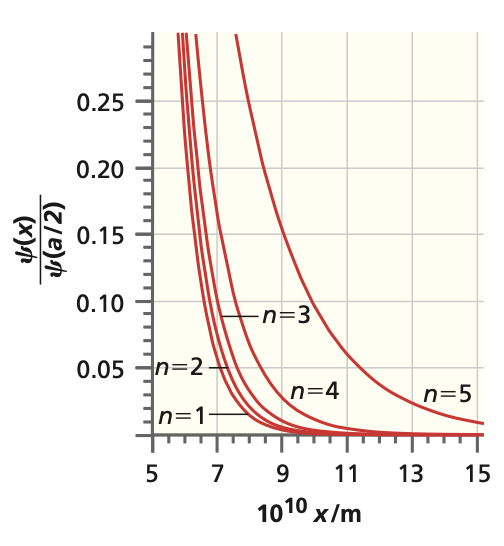
\includegraphics[width=0.9\linewidth,height=\textheight,keepaspectratio]{../../ch03/images/decay_psi.png}

}

\caption{Decay of a superposition, \(|\psi|^2\) evolving in time.}

\end{figure}%
\end{column}
\end{columns}

Superposition of energies \(\Rightarrow\) \textbf{motion} you can watch.
\end{block}
\end{frame}

\begin{frame}{Takeaway}
\protect\phantomsection\label{takeaway}
\begin{quote}
A single eigenstate only spins its phase, so nothing observable moves;
superpose different energies and their phases beat against each other,
and quantum dynamics comes alive.
\end{quote}
\end{frame}




\end{document}
